\documentclass[a4paper,12pt]{article}

\newif\ifen
\newif\ifpt

\newcommand{\en}[1]{\ifen#1\fi}
\newcommand{\pt}[1]{\ifpt#1\fi}

\ifdefined\english
  \entrue
\else
  \ifdefined\portuguese
    \pttrue
  \else
    % Change the following to switch the language
    % \entrue
    \pttrue
  \fi
\fi

\pt{\usepackage[brazil]{babel}}
\en{\usepackage{babel}}

\usepackage{amsthm, amsmath, amssymb, amsfonts, mathrsfs, mathtools}
\usepackage{xfrac, cancel}
\usepackage{seqsplit}
\usepackage{graphicx, setspace, xcolor, subcaption, svg}
\usepackage{float}
\usepackage[framemethod=TikZ]{mdframed}
\usepackage[bottom]{footmisc}
\usepackage[square,numbers]{natbib}
\usepackage{hyperref}
\usepackage{booktabs, diagbox, adjustbox, siunitx}
\usepackage{tabularx}
\usepackage{enumitem}
\usepackage{calc}
\usepackage[left=3cm,top=3cm,right=2cm,bottom=2cm]{geometry}
\pagestyle{myheadings}
\allowdisplaybreaks
\usepackage{setspace}
\usepackage{titlesec}
\usepackage{tocloft} % Package for customizing the table of contents
\usepackage{indentfirst}

\usepackage{setspace}
\setstretch{1.2}

\pt{
  \addto\captionsbrazil{
    \renewcommand{\proofname}{Prova} % Muda "demonstração" para "prova"
  }
}

% Commands
\renewcommand{\d}[1]{\ensuremath{\operatorname{d}\!{#1}}}
\DeclareMathOperator*{\esssup}{ess\,sup}
\DeclareMathOperator{\tr}{tr}
\DeclareMathOperator{\diag}{diag}
\renewcommand\qedsymbol{$\blacksquare$}
\newcommand{\textover}[2]{\overset{\mathclap{\scriptstyle #2}}{#1}}

\pt{
  \newtheorem*{theorem*}{Teorema}
  \newtheorem{theorem}{Teorema}
  \newtheorem{corollary}{Corolário}
  \newtheorem{conjecture}{Conjectura}

  \theoremstyle{definition}
  \newtheorem{example}{Exemplo}
  \newtheorem*{definition*}{Definição}
  \newtheorem{definition}{Definição}
  }
\en{
  \newtheorem*{theorem*}{Theorem}
  \newtheorem{theorem}{Theorem}
  \newtheorem{corollary}{Corollary}
  \newtheorem{conjecture}{Conjecture}

  \theoremstyle{definition}
  \newtheorem{example}{Example}
  \newtheorem*{definition*}{Definition}
  \newtheorem{definition}{Definition}
}

\renewcommand{\cftsecleader}{\cftdotfill{\cftdotsep}} % Adds dots for sections
\renewcommand{\cftsubsecleader}{\cftdotfill{\cftdotsep}} % Adds dots for subsections
\renewcommand{\cftsubsubsecleader}{\cftdotfill{\cftdotsep}} % Adds dots for subsubsections

\usepackage{fancyhdr}

% Set the page style to 'fancy'
\pagestyle{fancy}

% Clear all header and footer fields
\fancyhf{}

% Define the page number to appear at the center of the footer
\fancyfoot[C]{\thepage}

% Remove the header and footer lines (optional)
\renewcommand{\headrulewidth}{0pt}
\renewcommand{\footrulewidth}{0pt}

\fancyhf{} % Clear all header and footer fields
\fancyfoot[C]{\thepage} % Center the page number in the footer


\bibliographystyle{abbrvnat}

\begin{document}

\pagenumbering{gobble}
\begin{center}
  \textbf{INSTITUTO ALPHA LUMEN}\\
  \vspace{0.1cm}
  2° ANO DO ENSINO MÉDIO
\end{center}
\vspace{3cm}
\begin{center}
  Tiago Trindade\\
  Pedro Martineli
\end{center}
\vspace{8cm}
\begin{center}
  \large \textbf{Contagem de funções $k$-limitadas em $[n]$}
\end{center}
\vspace{8cm}
\begin{center}
  São José dos Campos-SP\\2024
\end{center}
\newpage

\begin{center}
  Tiago Trindade\\Pedro Martineli
\end{center}
\vspace{7cm}
\begin{center}
  \large \textbf{Contagem de funções $k$-limitadas em $[n]$}
\end{center}
\vspace{5cm}
\begin{flushright}
  \parbox{0.45\linewidth}{\sloppy
    Trabalho de Conclusão de Curso apresentado ao Instituto Alpha Lumen como parte das                 exigências para a obtenção do título de conclusão da 2ª série do Ensino Médio. \\[10pt]
    Orientador: Prof. Lucas Henrique \\[5pt]
    Supervisora: Prof. Ana Cecília Leal
  }
\end{flushright}
\vspace{4cm}
\begin{center}
  \normalsize São José dos Campos\\2024
\end{center}
\newpage

\vspace*{\fill}

\hspace{8cm}
\begin{minipage}{0.45\textwidth}
  \raggedright
  \pt{Dedicamos este trabalho ao professor Krerley Oliveira, cuja dedicação à educação é evidente em iniciativas como o Novo Ensino Suplementar. Seu apoio e orientações precisas foram cruciais, inspirando-nos continuamente à excelência.}
  \en{We dedicate this work to Professor Krerley Oliveira, whose dedication to education is evident in initiatives such as Novo Ensino Suplementar. His support and precise guidance were crucial, continuously inspiring us towards excellence.}
\end{minipage}

\begin{center}
  \large \textbf{
    \pt{Agradecimentos}
    \en{Acknowledgements}
  }
\end{center}

\par
\pt{Agradecemos profundamente ao professor Lucas Henrique, orientador deste trabalho, cuja expertise e direcionamento foram fundamentais para a elucidação e prova dos resultados aqui apresentados. Sua capacidade de guiar nossos esforços em meio aos desafios teóricos foi essencial para o sucesso deste estudo.}
\en{We deeply thank Professor Lucas Henrique, the advisor of this work, whose expertise and guidance were fundamental to the elucidation and proof of the results presented here. His ability to steer our efforts amidst theoretical challenges was essential for the success of this study.}

\pt{Expressamos nossa sincera gratidão aos nossos pais, que nos proporcionaram suporte constante e condições favoráveis para que seguíssemos com determinação em busca de nossos objetivos. Seu apoio incondicional e sua confiança em nossa capacidade foram pilares em nossa formação pessoal e acadêmica.}
\en{We express our sincere gratitude to our parents, who provided us with constant support and favorable conditions to pursue our goals with determination. Their unconditional support and trust in our abilities were pillars in our personal and academic development.}

\pt{Somos também gratos ao Novo Ensino Suplementar, que nos ofereceu uma base teórica robusta e indispensável, enriquecendo nosso conhecimento e ampliando nossa perspectiva acadêmica, o que foi crucial para o desenvolvimento deste trabalho.}
\en{We are also grateful to Novo Ensino Suplementar, which provided us with a robust and indispensable theoretical foundation, enriching our knowledge and broadening our academic perspective, which was crucial for the development of this work.}

\pt{Agradecemos ao Instituto Alpha Lumen por possibilitar um avanço significativo em nossa trajetória acadêmica. O suporte oferecido pelo instituto foi determinante, permitindo que nos dedicássemos ao aprofundamento nos estudos matemáticos, o que foi decisivo para nosso crescimento e realização acadêmica.}
\en{We thank Instituto Alpha Lumen for enabling significant advancement in our academic journey. The support offered by the institute was decisive, allowing us to dedicate ourselves to the deepening of mathematical studies, which was crucial for our academic growth and achievement.}

\pt{
  \begin{center}
  \large \textbf{Resumo}
\end{center}
\vspace{1cm}
\par Neste trabalho, estabelecemos a definição de funções $(\alpha, \lambda)$-limitadas, encontramos alguns resultados imediatos desta definição e descobrimos a caracterização assintótica da quantidade de funções $k$-limitadas em $[n]$ considerando a distância de Manhattan, utilizando ferramentas da combinatória algébrica, como matrizes de Toeplitz, e da teoria dos grafos.

\vspace{1cm}

\begin{raggedleft}
  \textbf{Palavras-chave}: Espaços Métricos; Matrizes de Toeplitz; Estimativas Assintóticas; Combinatória Algébrica; Teoria dos Grafos.
\end{raggedleft}
\newpage

  \begin{center}
  \large \textbf{Abstract}
\end{center}
\vspace{1cm}
\par In this work, we introduce the concept of $(\alpha, \lambda)$-bounded functions, characterized by limited local variation, which are especially useful in discrete sets. Initially, we formally define these functions and investigate their fundamental properties, highlighting significant differences from continuous functions. The main result obtained is the asymptotic characterization of $a(n, k)$, representing the number of functions from $[n]$ to $[n]$ that are $k$-bounded with respect to Manhattan distance. The proof of this result combines Toeplitz matrices with a well-known inequality from graph theory. Additionally, we emphasize the relevance of the intersection between algebraic combinatorics, graph theory, and the analysis of discrete metric spaces, suggesting future research into the topological properties of these functions and their potential applications in computational and mathematical contexts.

\vspace{1cm}

\begin{raggedleft}
  \textbf{Keywords-chave}: metric spaces; Toeplitz matrices; asymptotic estimates; graph theory; algebraic combinatorics.
\end{raggedleft}

}
\en{
  \begin{center}
  \large \textbf{Abstract}
\end{center}
\vspace{1cm}
\par In this work, we introduce the concept of $(\alpha, \lambda)$-bounded functions, characterized by limited local variation, which are especially useful in discrete sets. Initially, we formally define these functions and investigate their fundamental properties, highlighting significant differences from continuous functions. The main result obtained is the asymptotic characterization of $a(n, k)$, representing the number of functions from $[n]$ to $[n]$ that are $k$-bounded with respect to Manhattan distance. The proof of this result combines Toeplitz matrices with a well-known inequality from graph theory. Additionally, we emphasize the relevance of the intersection between algebraic combinatorics, graph theory, and the analysis of discrete metric spaces, suggesting future research into the topological properties of these functions and their potential applications in computational and mathematical contexts.

\vspace{1cm}

\begin{raggedleft}
  \textbf{Keywords-chave}: metric spaces; Toeplitz matrices; asymptotic estimates; graph theory; algebraic combinatorics.
\end{raggedleft}

  \begin{center}
  \large \textbf{Resumo}
\end{center}
\vspace{1cm}
\par Neste trabalho, estabelecemos a definição de funções $(\alpha, \lambda)$-limitadas, encontramos alguns resultados imediatos desta definição e descobrimos a caracterização assintótica da quantidade de funções $k$-limitadas em $[n]$ considerando a distância de Manhattan, utilizando ferramentas da combinatória algébrica, como matrizes de Toeplitz, e da teoria dos grafos.

\vspace{1cm}

\begin{raggedleft}
  \textbf{Palavras-chave}: Espaços Métricos; Matrizes de Toeplitz; Estimativas Assintóticas; Combinatória Algébrica; Teoria dos Grafos.
\end{raggedleft}
\newpage

}
\section*{Notações}
% \addcontentsline{toc}{section}{Notações}

\begin{description}[leftmargin=!, labelwidth=\widthof{\texttt{Função $f : X \to Y$}}]
  \item[{$[n]$}] Conjunto $\{1, 2, \dots, n\}$.

  \item[$\mathbb{Z}_{>0}$] Conjunto dos inteiros positivos.

  \item[$(X, d_X)$] Espaço métrico $X$ com a métrica $d_X$.

  \item[$\mathbf{1}_n$] Vetor coluna de dimensão $n$ com todos os elementos iguais a $1$.

  \item[$(v)_i$] O $i$-ésimo elemento de um vetor $v$.

  \item[$\| \cdot \|_2$] Norma espectral de uma matriz ou vetor.

  \item[$H^2(\mathbb{T})$] Espaço de Hardy das funções analíticas na circunferência unitária $\mathbb{T}$.

  \item[$T(a)$] Operador de Toeplitz com símbolo $a \in L^\infty(\mathbb{T})$, definido por $T(a)f = P(af)$ onde $P$ é a projeção de Szegő.

  \item[$\sigma(T(a))$] Espectro do operador de Toeplitz $T(a)$.

  \item[$\{a_n\}$] Sequência indexada por \( n \in \mathbb{Z} \), ou seja, uma sequência de termos \( \{a_n : n \in \mathbb{Z}\} \) onde \( n \) varia em todos os inteiros.

  \item[$\Lambda$] Matriz diagonal resultante da diagonalização de uma matriz circulante através da matriz de Fourier.

  \item[$D_k(t)$] Kernel de Dirichlet de ordem $k$.

  \item[$T_n(a)$] Matriz de Toeplitz $n \times n$ gerada pelo símbolo $a \in L^\infty(\mathbb{T})$.

  \item[$l^2(\mathbb{Z}_{> 0})$] Espaço de sequências quadrado-somáveis indexadas por $\mathbb{Z}_{> 0}$.

  \item[$a(x)$] Função símbolo associada a uma matriz de Toeplitz, geralmente definida como um polinômio trigonométrico.

  \item[$L^\infty(\mathbb{T})$] Espaço das funções definidas na circunferência unitária complexa $\mathbb{T}$ essencialmente limitadas.

  \item[$\esssup$] Supremo essencial.

  \item[$\overline{B}_{\lambda}(x)$] Bola fechada de raio $\lambda$ centrada em $x$ no espaço métrico considerado.

  \item[$a(n) \sim b(n)$] $a(n)$ e $b(n)$ são assintoticamente equivalentes, isto é, $\lim_{n \to \infty} \frac{a(n)}{b(n)} = 1$.

  \item[$f \in L^1(\mathbb{T})$] Função $f$ integrável definida na circunferência unitária $\mathbb{T}$.

  \item[$\mathcal{O}(\cdot)$] Notação Big-O, indicando que uma função $f(n)$ cresce no máximo na ordem de outra função $g(n)$, ou seja, $f(n) = \mathcal{O}(g(n))$ se existem constantes $C, n_0 > 0$ tais que $|f(n)| \leq C \cdot |g(n)|$ para todo $n \geq n_0$.
\end{description}

\tableofcontents

\newpage

\pagenumbering{arabic}
\setcounter{page}{8}

\phantomsection
\section*{
  \pt{Introdução}
  \en{Introduction}
 }
\addcontentsline{toc}{section}{
  \pt{Introdução}
  \en{Introduction}
} % Adds "Introduction" to the ToC without a chapter number
\vspace{1cm}

\normalsize

\pt{É fato conhecido que toda função definida em um subconjunto discreto de $\mathbb{R}$ é contínua considerando a norma induzida. Desta forma, o conceito de continuidade não é muito útil ao analisar funções definidas em conjuntos discretos, motivando assim a introdução de um novo conceito, que chamaremos de funções $(\alpha,\lambda)$-limitadas.}
\en{It is a well-known fact that every function defined on a discrete subset of $\mathbb{R}$ is continuous when considering the induced norm. Thus, the concept of continuity is not very useful when analyzing functions defined on discrete sets, thereby motivating the introduction of a new concept we call $(\alpha,\lambda)$-bounded functions.}

\pt{A introdução de propriedades alternativas para funções em espaços discretos não é inédita na literatura matemática. Conceitos como funções de variação limitada e funções de descontinuidade controlada têm sido explorados para analisar comportamentos específicos em contextos combinatórios e algorítmicos (veja por exemplo \cite{Rosenfeld}). No entanto, as funções $(\alpha,\lambda)$-limitadas se distinguem por sua flexibilidade em parametrizar a restrição de variação, permitindo uma análise mais granular.}
\en{The introduction of alternative properties for functions in discrete spaces is not new in mathematical literature. Concepts such as bounded variation functions and controlled discontinuity functions have been explored to analyze specific behaviors in combinatorial and algorithmic contexts (see, for example, \cite{Rosenfeld}). However, $(\alpha,\lambda)$-bounded functions distinguish themselves by their flexibility in parameterizing variation constraints, allowing for a more granular analysis.}

\pt{Além disso, a utilização de matrizes de Toeplitz na análise de propriedades funcionais tem sido amplamente estudada em áreas como processamento de sinais e teoria dos operadores, como mostrado em \cite{GrenanderSzego}. Trabalhos como \cite{bottcher} demonstram a eficácia dessas matrizes na caracterização de operadores e na obtenção de estimativas assintóticas. Este estudo aproveita essas ferramentas para investigar a contagem assintótica de funções $(k,1)$-limitadas, estabelecendo mais uma ponte entre essas áreas aparentemente distintas.}
\en{Furthermore, the use of Toeplitz matrices in analyzing functional properties has been extensively studied in areas such as signal processing and operator theory, as shown in \cite{GrenanderSzego}. Works like \cite{bottcher} demonstrate the effectiveness of these matrices in characterizing operators and obtaining asymptotic estimates. This study leverages these tools to investigate the asymptotic counting of $(k,1)$-bounded functions, thereby establishing another bridge between these seemingly distinct areas.}

\pt{No âmbito da ciência da computação, onde as funções frequentemente operam em espaços discretos e finitos, como alocação de memória, compressão de dados e processamento de sinais digitais, a introdução das funções $(\alpha,\lambda)$-limitadas fornece outra ferramenta para formalizar e analisar a estabilidade e robustez de algoritmos e sistemas. Elas podem ser particularmente vantajosas em cenários onde variações leves de entrada devido a fatores como ruído, erros de compressão de dados ou pequenas perturbações nos processos computacionais não devem afetar desproporcionalmente as saídas.}
\en{In the realm of computer science, where functions often operate on discrete and finite spaces, such as memory allocation, data compression, and digital signal processing, the introduction of $(\alpha,\lambda)$-bounded functions provides another tool to formalize and analyze the stability and robustness of algorithms and systems. They might be particularly advantageous in scenarios where slight input variations due to factors like noise, data compression errors, or minor perturbations in the computational processes should not disproportionately affect the outputs.}

\pt{A capacidade de contar e caracterizar funções definidas em espaços discretos com restrições específicas, como as impostas pelas funções $(\alpha,\lambda)$-limitadas, é crucial para o desenvolvimento de resultados que exigem controle preciso sobre a variação das funções. Além disso, a análise assintótica da quantidade de funções $(k,1)$-limitadas fornece ideias valiosas sobre o comportamento de sistemas discretos à medida que seu tamanho cresce, permitindo a identificação de padrões e tendências que podem não ser evidentes em análises de casos específicos. Essa compreensão é essencial para o avanço de teorias combinatórias e para a resolução de problemas que envolvem grandes estruturas discretas. O uso de matrizes de Toeplitz e a aplicação da teoria dos grafos neste contexto destacam a combinação de diferentes áreas necessária para abordar problemas complexos em matemática.}
\en{The ability to count and characterize functions defined on discrete spaces with specific constraints, such as those imposed by $(\alpha,\lambda)$-bounded functions, is crucial for developing results that require precise control over function variation. Additionally, the asymptotic analysis of the number of $(k,1)$-bounded functions provides valuable insights into the behavior of discrete systems as their size grows, allowing the identification of patterns and trends that may not be evident in analyses of specific cases. This understanding is essential for advancing combinatorial theories and for solving problems involving large discrete structures. The use of Toeplitz matrices and the application of graph theory in this context highlight the combination of different areas necessary to address complex problems in mathematics.}

\pt{No primeiro capítulo, introduzimos essa nova definição, mostramos alguns exemplos e provamos resultados simples que mostram o contraste entre funções $(\alpha,\lambda)$-limitadas e funções contínuas.}
\en{In the first chapter, we introduce this new definition, present some examples, and prove simple results that highlight the contrast between $(\alpha,\lambda)$-bounded functions and continuous functions.}

\pt{No segundo capítulo, introduzimos a definição de matrizes de Toeplitz, juntamente com resultados relevantes que são empregados no terceiro capítulo, assim como em possíveis generalizações dos teoremas apresentados nele.}
\en{In the second chapter, we introduce the definition of Toeplitz matrices, along with relevant results that are employed in the third chapter, as well as in possible generalizations of the theorems presented therein.}

\pt{No terceiro capítulo, estendemos um resultado de \cite{coulson} ao encontrar a caracterização assintótica da quantidade de funções $(k,1)$-limitadas em $[n]$:}
\en{In the third chapter, we extend a result from \cite{coulson} by finding the asymptotic characterization of the number of $(k,1)$-bounded functions on $[n]$:}

\begin{theorem*}
  \pt{Seja $k \ge 0$ um inteiro fixo, e seja $a(n, k)$ a quantidade de funções $k$-limitadas de $[n]\to[n]$. Então, $a(n,k) \sim n(2k+1)^{n-1}$.}
  \en{Let $k \ge 0$ be a fixed integer, and let $a(n, k)$ be the number of $k$-bounded functions from $[n] \to [n]$. Then, $a(n,k) \sim n(2k+1)^{n-1}$.}
\end{theorem*}

\pt{Este resultado é provado usando propriedades de matrizes de Toeplitz e uma cota bem conhecida da teoria dos grafos.}
\en{This result is proven using properties of Toeplitz matrices and a well-known bound from graph theory.}

\pt{Por fim, no apêndice apresentamos alguns resultados interessantes acerca de matrizes de Toeplitz.}
\en{Finally, in the appendix, we present some interesting results concerning Toeplitz matrices.}

\pt{Desejamos com este trabalho mostrar como uma combinação de matrizes de Toeplitz e teoria dos grafos podem ser usadas para obter estimativas assintóticas precisas de quantidades como a estudada neste trabalho: o número funções $k$-limitadas de $[n]$ para $[n]$.}
\en{With this work, we aim to demonstrate how a combination of Toeplitz matrices and graph theory can be used to obtain precise asymptotic estimates of quantities such as those studied in this work: the number of $k$-bounded functions from $[n]$ to $[n]$.}

\section{Definições}
\vspace{1cm}
A definição de $(\alpha,\lambda)$-limitada é inicialmente apresentada como uma propriedade pontual, assim como a definição de continuidade: \begin{definition} Sejam $\alpha, \lambda \ge 0$, $(X, d_X)$ e $(Y, d_Y)$ espaços métricos, $\mathcal{X} \subseteq X$. Uma função $f : \mathcal{X} \to Y$ é dita \textit{$(\alpha,\lambda)$-limitada no ponto $x \in \mathcal{X}$} quando, para todo $\tilde{x} \in \mathcal{X}$ tal que $d_X(x, \tilde{x}) \le \lambda$, temos $d_Y(f(x), f(\tilde{x})) \le \alpha$. \end{definition}

\begin{figure}[h!]
  \begin{center}
    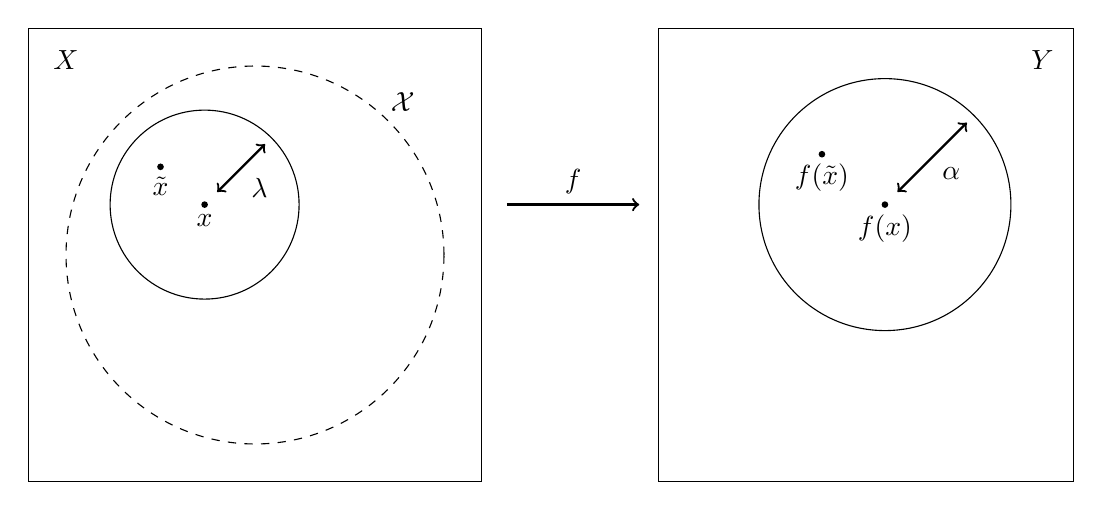
\begin{tikzpicture}[scale=.8]
      \node (X) at (-3, 3.1) {$X$};
      \node (Y) at (12.5, 3.1) {$Y$};

      \draw (-3.6, -3.6) rectangle (3.6, 3.6);
      \draw (6.4, -3.6) rectangle (13, 3.6);

      \fill (-0.8, 0.8) circle (1.5pt);
      \node[below] (x) at (-0.8, 0.8) {$x$};

      \fill (-1.5, 1.4) circle (1.5pt);
      \node[below] (xt) at (-1.5, 1.4) {$\tilde{x}$};

      \fill (10, 0.8) circle (1.5pt);
      \fill (9.0, 1.6) circle (1.5pt);
      \node[below] (y) at (10, 0.8) {$f(x)$};
      \node[below] (yt) at (9.0, 1.6) {$f(\tilde{x})$};

      \draw[dashed] (0, 0) ellipse (3cm and 3cm) node[above right, xshift=1.6cm, yshift=1.7cm] {$\mathcal{X}$};
      \draw[] (-0.8, 0.8) ellipse (1.5cm and 1.5cm);
      \draw[<->, thick] (-0.6, 1) -- ++(0.76, 0.76) node[midway, below right] {$\lambda$};
      \draw[] (10, 0.8) ellipse (2cm and 2cm);
      \draw[<->, thick] (10.2, 1) -- ++(1.1, 1.1) node[midway, below right] {$\alpha$};
      \draw[->, thick] (4, 0.8) -- (6.1, 0.8) node[midway, above] {$f$};
    \end{tikzpicture}
  \end{center}
  \captionsetup{justification=centering}
  \caption{
    \pt{Função $f : \mathcal{X} \to Y$ $(\alpha, \lambda)$-limitada em $x$.}
    \en{Function $f : \mathcal{X} \to Y$ which is $(\alpha, \lambda)$-bounded at $x$.}
  }
\end{figure}

\vspace{1cm}

\begin{definition} Sejam $\alpha, \lambda \ge 0$, $(X, d_X)$ e $(Y, d_Y)$ espaços métricos, $\mathcal{X} \subseteq X$. Uma função $f : \mathcal{X} \to Y$ é dita \textit{$(\alpha,\lambda)$-limitada} quando, para todo $x$ em $\mathcal{X}$, $f$ é $(\alpha,\lambda)$-limitada no ponto $x$. \end{definition}

Note que, para $\lambda = 1$, a definição acima estende naturalmente a condição de Hölder para a ordem $0$ e coeficiente $\alpha$ (veja \cite{holder}). Também é importante notar que muitos resultados de funções contínuas não se estendem para funções $(\alpha, \lambda)$-limitadas. Veja o exemplo \ref{vitali}.

Ao alterar a métrica, podemos considerar $\lambda = 1$ na definição acima sem perda de generalidade, porque $(X, d_X)$ é um espaço métrico se, e somente se, $(X, \lambda d_X)$ é um espaço métrico para todo $\lambda > 0$. Se desejarmos ter $d_X(x, \tilde{x}) \le \lambda$ para algum $\lambda > 0$, então podemos considerar o espaço métrico $(X, \frac{1}{\lambda} d_X)$ ao invés de $(X, d_X)$. Como nosso principal interesse neste trabalho são as funções $(k,1)$-limitadas, usaremos $\alpha$-limitada para denotar $(\alpha,1)$-limitada.

\begin{example} \label{vitali} Considere $V$ um conjunto de Vitali. A função $f : [0, 1] \to \mathbb{R}$, definida por $f(x) = 1_V$ se $x \in (0, 1)$ e $f(x) = 1 - x$ caso contrário, é $1$-limitada (considerando a métrica usual) mas não é contínua, não possui pontos fixos e não é Lebesgue integrável (veja \cite{vitali}). \end{example}

Toda função $f : X \to \mathbb{R}$ definida em um subconjunto discreto de $\mathbb{R}$ é contínua considerando a métrica induzida por $\mathbb{R}$, mas pode não ser $\alpha$-limitada para qualquer $\alpha > 0$. Veja a seguir.

\begin{example} \label{two_to_n} $f : \mathbb{Z} \to \mathbb{Z}$ dada por $n \mapsto 2^n$ não é $\alpha$-limitada (considerando a métrica usual) para nenhum $\alpha > 0$, pois $f(n + 1) - f(n) = 2^{n}$ é ilimitada. \end{example}

Abaixo estão alguns resultados imediatos da definição de $\alpha$-limitado.

\begin{theorem} Toda função $\alpha$-limitada é $(\alpha+\epsilon)$-limitada para todo $\epsilon > 0$. \end{theorem} \begin{proof} Evidente. \end{proof}

\begin{theorem} Sejam $(X, d_X)$ e $(Y, d_Y)$ espaços métricos, $\mathcal{X} \subseteq X$. Toda função Lipschitz contínua, com constante $K$, $f : \mathcal{X} \to Y$ é $K$-limitada. \end{theorem} \begin{proof} Para todo $x_1 \in \mathcal{X}$, $x_2 \in \mathcal{X}, d_X(x_1, x_2) \le 1$ e consequentemente $d_Y(f(x_1), f(x_2)) \le K d_X(x_1, x_2) \le K$. \end{proof}
Note que nem todas as funções $\alpha$-Hölder contínuas são $\beta$-limitadas para algum $\beta > 0$. A função $\sqrt{\cdot} : \mathbb{R}^+ \to \mathbb{R}$ constitui um contraexemplo (considerando a métrica usual) pelo mesmo motivo mencionado no exemplo \ref{two_to_n}.

\begin{theorem} Sejam $(X, d_X)$ e $(Y, d_Y)$ espaços métricos, $\mathcal{X} \subseteq X$, e $f : \mathcal{X} \to Y$ uma função. Se para todo $\epsilon > 0$ existe um $\alpha \in (0, \epsilon]$ tal que $f$ é $\alpha$-limitada, então $f$ é contínua. \end{theorem} \begin{proof} Com efeito, para cada $x \in \mathcal{X}, \epsilon > 0$, existe algum $\alpha \in (0, \epsilon]$ tal que $\tilde{x} \in \mathcal{X}, d_X(x, \tilde{x}) \le 1 \implies d_Y(f(x), f(\tilde{x})) \le \alpha \le \epsilon$. \end{proof}

\begin{theorem}
  Sejam $(X, d_X)$ e $(Y, d_Y)$ espaços métricos, $\mathcal{X} \subseteq X$. Se $(f_n) \to f$ ponto a ponto, $f_n : \mathcal{X} \to Y$ são $\alpha$-limitadas para todo $n \in \mathbb{Z}_{> 0}$, então $f$ é $\alpha$-limitada.
\end{theorem}
\begin{proof}
  Suponha, por contradição, que $f$ não seja $\alpha$-limitada. Então existem $x_1, x_2 \in \mathcal{X}$, $d_X(x_1, x_2) \le 1$, tal que $d_Y(f(x_1), f(x_2)) \coloneqq k > \alpha$. Como $(f_n) \to f$ ponto a ponto, existe algum $n \in \mathbb{Z}_{> 0}$ com $d_Y(f_n(x_1), f(x_1)) < \frac{k - \alpha}{2}$ e $d_Y(f_n(x_2), f(x_2)) < \frac{k - \alpha}{2}$. Consequentemente, $d_Y(f_n(x_1), f_n(x_2)) > k - \frac{k - \alpha}{2} - \frac{k - \alpha}{2} = \alpha$, uma contradição.
\end{proof}

As funções $\alpha$-limitadas podem não ser o limite pontual de qualquer sequência de funções contínuas.

\begin{example} A função de Dirichlet $1_\mathbb{Q} : [0, 1] \to \mathbb{R}$, também como função indicadora dos racionais, é $1$-limitada considerando a métrica usual de $\mathbb{R} \supset [0, 1]$, mas não é o limite pontual de nenhuma sequência de funções contínuas, pois é uma função da classe 2 de Baire (veja \cite{baire}). \end{example}

A aritmética com funções $\alpha$-limitadas não é a mesma que com funções contínuas definidas em $\mathbb{R}$.

\begin{theorem}
  Sejam $(X, d_X)$ e $(Y, d_Y)$ espaços métricos e $(Y, +Y, \cdot_Y)$ um espaço vetorial sobre $\mathbb{R}$. Se $f : X \to Y$ e $g : X \to Y$ são duas funções $\alpha$-limitadas, então $f + g$ é $(2\alpha)$-limitada e $\gamma f$ é $(\gamma \alpha)$-limitada para todo $\gamma > 0$.
\end{theorem}
\begin{proof}
  Se $x \in X$ e $\tilde{x} \in X$, $d_X(x, \tilde{x}) \le 1$, então $f(\tilde{x}) \in \overline{B}_{\alpha}(f(x))$ e $g(\tilde{x}) \in \overline{B}_{\alpha}(g(x))$, portanto $(f + g)(\tilde{x}) = f(\tilde{x}) + g(\tilde{x}) \in \overline{B}_{2\alpha}((f + g)(x))$, e consequentemente $f + g$ é $(2\alpha)$-limitada. Analogamente, $(\gamma f)(\tilde{x}) \in \overline{B}_{\gamma \alpha}(f(x))$ e $\gamma f$ é $(\gamma \alpha)$-limitada.
\end{proof}

O teorema acima permite considerar espaços vetoriais de mapas entre dois espaços métricos que são $\alpha$-limitados para algum $\alpha \ge 0$.

O produto de duas funções $\alpha$-limitadas (com o mesmo domínio e contradomínio) pode não ser $\beta$-limitado para nenhum $\beta > 0$, assim como o recíproco de uma função $\alpha$-limitada (quando definido).

\begin{example} $f : \mathbb{Z}_{> 0} \to \mathbb{Z}_{> 0}$ dada por $f(n) = n$ é $1$-limitada (considerando a métrica usual), mas $f^2$ coincide com $g : \mathbb{R} \to \mathbb{R}$, $g(x) = x^2$, portanto não é $\alpha$-limitada para nenhum $\alpha > 0$. \end{example}

\begin{example} $f : [1, +\infty) \to \mathbb{R}$ dada por $f(x) = \frac{1}{x^2}$ é $1$-limitada, mas $\frac{1}{f}$ coincide com $g : \mathbb{R} \to \mathbb{R}$, $g(x) = x^2$, portanto não é $\alpha$-limitada para nenhum $\alpha > 0$. \end{example}

O teorema de extensão para funções $\alpha$-limitadas não é muito forte.

Os exemplos abaixo ilustram por que as condições do teorema são necessárias.

\begin{example} Seja $X \coloneqq \{(x, \pm 1) \mid x \in \mathbb{Z}\} \subset \mathbb{Z}^2$. Considere $f : X \to \mathbb{Z}$ dada por $f(x, 1) = x$ e $f(x, -1) = 0$ para qualquer $x \in \mathbb{Z}$. Claramente, $f$ é $1$-limitada, considerando a métrica usual, mas $f$ não tem nenhuma extensão $\alpha$-limitada, para qualquer $\alpha > 0$, ao conjunto $\{(x, y) \mid x \in \mathbb{Z}, y \in \{-1,0,1\}\}$, pois $\overline{B}_1((x, 0)) \supset \{ (x, 1), (x, -1) \}$ e $f(x, 1) = x$, $f(x, -1) = 0$. \end{example}

\begin{figure}[H]
  \begin{center}
    \centering
    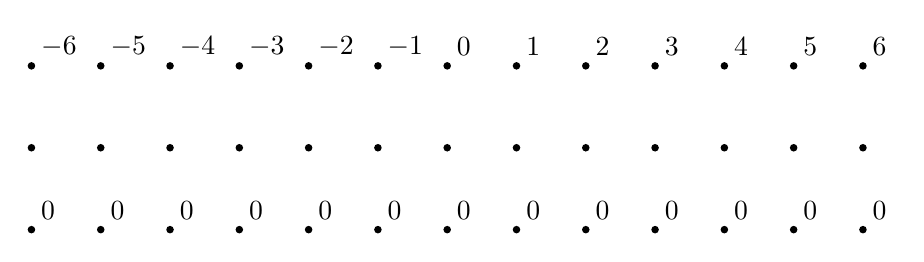
\begin{tikzpicture}[scale=0.8]
      \foreach \y in {1, 0, -1} {
          \foreach \x in {-6, ..., 6} {
              \fill[color=black] (\x*1.1+3,\y*1.3) circle (0.06);

              \ifnum\y=1
                \node[right] at (\x*1.1+3,\y*1.3+0.3) {$\x$};
              \fi
              \ifnum\y=-1
                \node[right] at (\x*1.1+3,\y*1.3+0.3) {$0$};
              \fi
            }
        }
    \end{tikzpicture}
    \captionsetup{justification=centering}
    \caption{
      \pt{Função $1$-limitada sem extensão $\alpha$-limitada, para qualquer $\alpha > 0$, para um conjunto com infinitos pontos adicionais.}
      \en{$1$-bounded function without an $\alpha$-bounded extension, for any $\alpha > 0$, for a set with infinitely many additional points.}
    }
  \end{center}
\end{figure}


\begin{example} Seja $s_n \in l^2(\mathbb{Z}_{> 0})$ a sequência com um $1$ na posição $n$-ésima e $0$'s nas outras posições, e $X = \{ s_n \mid n \in \mathbb{Z}_{> 0} \}$. $f : X \to \mathbb{Z}$ dada por $f(s_n) = n$ é $1$-limitada considerando a norma euclideana $l^2$, mas não tem nenhuma extensão $\alpha$-limitada ao conjunto $X \cup \{(0, 0, 0, \dots)\}$ para qualquer $\alpha \ge 0$. \end{example}

\begin{figure}[H]
  \begin{center}
    \begin{tikzpicture}
      \fill (0,0) circle (0.07);
      \node at ([shift={(1cm, -0.5cm)}] 0,0) {$(0, 0, \dots)$};

      % Constants
      \def\n{10} % Number of surrounding points
      \def\k{3.2}  % Constant k in the angle formula
      \def\startOffset{-77}

      % Loop to place points in a circular arrangement
      \foreach \i in {1,...,\n} {
          % Calculate angle for the point using (2 * pi / k) * log(N)
          \pgfmathsetmacro{\angle}{\startOffset + (360 / \k) * ln(\i + 1)}
          \pgfmathsetmacro{\angleout}{\startOffset + (360 / \k) * ln(\i)}


          % Coordinates of the surrounding point at radius 2
          \path (\angle:5) coordinate (P\i);
          \draw[dashed] (0, 0) -- (P\i);
          \ifnum\i>1
            \pgfmathtruncatemacro{\prev}{\i-1}
            % Calculate the start and end angles for each arc
            \pgfmathsetmacro{\startAngle}{\startOffset + (360 / \k) * ln(\prev + 1)}
            \pgfmathsetmacro{\endAngle}{\angle}
            \ifnum\i<4
              \draw[dashed]
              (P\prev) arc[start angle=\startAngle, end angle=\endAngle, radius=5]
              node[midway, above right] {\(\sqrt{2}\)}; % Label at midpoint of each edge
            \else
              \ifnum\i>4
                \draw[dashed]
                (P\prev) arc[start angle=\startAngle, end angle=\endAngle, radius=5];
              \else
                \draw[dashed]
                (P\prev) arc[start angle=\startAngle, end angle=\endAngle, radius=5]
                node[midway, above] {\(\sqrt{2}\)}; % Label at midpoint of each edge
              \fi
            \fi
          \fi


          % Draw the point and label it
          %\fill (P\i) circle (0.05) node[below left] {$s_{\i}$};

          \ifnum\i<5
            \fill[font=\bfseries] (P\i) circle (0.05) node[above left] {$s_{\i}$};
          \else
            \ifnum\i>9
              \fill (P\i) circle (0.05) node[below] {$s_{\i}$};
            \else
              \fill (P\i) circle (0.05) node[below left] {$s_{\i}$};
            \fi
          \fi
        }

      \node at ([shift={(0.5cm, -0.7cm)}] P10) {$\ddots$};

    \end{tikzpicture}
    \captionsetup{justification=centering}
    \caption{Sequência de pontos de $l^2(\mathbb{Z}_{> 0})$ na esfera unitária. A escala dos angulos que os pontos $s_n$ formam com o eixo $x$ é logarítimica em $n$.}
  \end{center}
\end{figure}


\begin{theorem} \label{tietze}
  Sejam $(X,d_X)$ e $(Y, d_Y)$ espaços métricos, $\mathcal{X}, \tilde{\mathcal{X}} \subset X$, onde $\tilde{\mathcal{X}}$ é finito, e seja $f : \mathcal{X} \to Y$ uma função $(\alpha,\lambda)$-limitada. Existe $\beta \ge 0$ tal que $f$ tem uma extensão $(\beta,\lambda)$-limitada para $\mathcal{X} \cup \tilde{\mathcal{X}}$ se e somente se $f$ é limitada em $\overline{B}_{\lambda}(\tilde{x}) \cap \mathcal{X}$ para cada $\tilde{x} \in \tilde{\mathcal{X}}$.
\end{theorem}

\begin{proof} A necessidade dessa condição é evidente. Vamos então provar que ela é suficiente.

  Podemos supor que $\tilde{\mathcal{X}} \cap \mathcal{X} = \varnothing$, já que obviamente $f$ é limitada em $\overline{B}_{\lambda}(x)$ para cada $x \in \mathcal{X}$.

  Procederemos por indução sobre o número $n$ de elementos em $\tilde{\mathcal{X}}$.

  Para $n = 0$, o resultado é óbvio. Suponha que o resultado seja verdade para $n$, e $\tilde{\mathcal{X}}$ tenha $n+1$ elementos.

  Fixe $\tilde{x} \in \tilde{\mathcal{X}}$ e $y \in Y$. Por hipótese, $f$ tem uma extensão $(\beta,\lambda)$-limitada para $\mathcal{X} \cup (\tilde{\mathcal{X}} \setminus {\tilde{x}})$. Defina $\tilde{f} : \mathcal{X} \cup \tilde{\mathcal{X}}$ por $\tilde{f}(\tilde{x}) = y$ e $\tilde{f}(x) = f(x)$ para cada $x \in \mathcal{X} \cup (\tilde{\mathcal{X}} \setminus {\tilde{x}})$. Claramente existe $\gamma \ge 0$ tal que $\tilde{f}$ é $(\gamma,\lambda)$-limitada em $x$ para cada $x$ diferente de $\tilde{x}$. Mas como $f$ é limitada em $\overline{B}_{\lambda}(\tilde{x}) \cap \mathcal{X}$, existe $M \ge 0$ tal que $\lvert f(x) \rvert \le M$ para cada $x \in \overline{B}_{\lambda}(\tilde{x}) \cap \mathcal{X}$. Portanto, $\lvert \tilde{f}(x)-\tilde{f}(\tilde{x})\rvert \le \lvert f(x)\rvert + \lvert -y\rvert \le M + \lvert-y\rvert$ para cada $x \in \overline{B}_{\lambda}(\tilde{x}) \cap \mathcal{X}$, e consequentemente, $\tilde{f}$ é $(\max\{M + \lvert-y\rvert, \gamma\},\lambda)$-limitada. Assim, o resultado também segue para $n+1$.
\end{proof}

Este corolário e os exemplos subsequentes ilustram algumas propriedades interessantes das funções $\alpha$-limitadas, especialmente como elas podem ser estendidas de um conjunto compacto para incluir finitos pontos adicionais.

\begin{corollary} Toda função $\alpha$-limitada definida em um conjunto compacto $\mathcal{X}$ possui uma extensão $\beta$-limitada para qualquer conjunto $\tilde{\mathcal{X}} \supseteq \mathcal{X}$ tal que $\tilde{\mathcal{X}} \setminus \mathcal{X}$ é finito. \end{corollary}

\begin{proof} Como $\mathcal{X}$ é compacto, o conjunto $\{ \overline{B}_1(x) \mid x \in \mathcal{X} \} \supseteq \mathcal{X}$ possui uma subcobertura finita, que naturalmente também cobre $\overline{B}_1(x) \cap \mathcal{X} \subset \mathcal{X}$ para todos os $x \in \tilde{\mathcal{X}} \setminus \mathcal{X}$. Assim pode-se tomar $\beta$ como o maior valor entre $\alpha$ e a variação máxima da extenção em cada um dos pontos adicionados. \end{proof}

Note que podemos ter $\beta < \alpha$ no teorema acima, já que $\alpha$ não precisa ser mínimo e $\tilde{\mathcal{X}} \setminus \mathcal{X}$ pode, por exemplo, ser vazio. Também não podemos assumir que $\beta = \alpha$ no teorema acima.

\begin{example} Seja $X \coloneqq \{-1, 1\} \subset \mathbb{Z}$. A função $f : X \to \mathbb{Z}$ dada por $f(x) = 2x$ é $1$-limitada (considerando a métrica usual), mas não existe uma extensão $1$-limitada de $f$ para o conjunto $\{-1, 0, 1\}$. \end{example}

O que foi apresentado neste capítulo mostra as propriedades básicas das funções $(\alpha,\lambda)$-limitadas e como elas se comportam em comparação com funções contínuas em espaços métricos. Os teoremas e exemplos ilustram as características fundamentais dessas funções, e fornecem uma base para o estudo aprofundado das funções $(\alpha,\lambda)$-limitadas em contextos mais específicos, como o explorado no terceiro capítulo.

\section{Resultados da teoria de matrizes de Toeplitz} \vspace{1cm}

\par Em \cite{Toeplitz1911} Otto Toeplitz apresenta as $L$-formas, anteriormente estudadas em sua tese de habilitação para a universidade Universidade de Göttingen. Posteriormente seus estudos foram adaptados para o que hoje chamamos de matrizes de Toeplitz.

Uma matriz de Toeplitz é uma matriz com entradas complexas possivelmente infinita da forma \[ \begin{pmatrix} a_{0} & a_{-1} & a_{-2} & \cdots \\ a_{1} & a_{0} & a_{-1} & \cdots \\ a_2 & a_{1} & a_{0} & \cdots \\ \vdots & \vdots & \vdots & \ddots \end{pmatrix}\text{.} \]

As matrizes de Toeplitz possuem uma ampla gama de aplicações, que vão desde teoria dos operadores, análise harmonica, teoria da informação e processamento de sinais à mecânica quântica.

Essas matrizes são especialmente úteis quando a sequência $\{a_n\}$ determina os coeficientes de Fourier de uma determinada função, uma vez que isso possibilita utilizar ferramentas da análise para calcular, por exemplo, a norma do operador em $l^2(\mathbb{Z}_{> 0})$ que a matriz representa.

Em \cite{Toeplitz1911} Toeplitz mostra uma condição necessária e suficiente para que uma matriz de Toeplitz induza um operador limitado em $l^2(\mathbb{Z}_{> 0})$, é claro, utilizando a linguagem das $L$-formas.

\begin{theorem*}[Operadores limitados induzidos por matrizes de Toeplitz]
  A matriz infinita \[A = \begin{pmatrix} a_{0} & a_{-1} & a_{-2} & \cdots \\ a_{1} & a_{0} & a_{-1} & \cdots \\ a_2 & a_{1} & a_{0} & \cdots \\ \vdots & \vdots & \vdots & \ddots \end{pmatrix}\] induz um operador limitado em $l^2(\mathbb{Z}_{>0})$ se e somente se os números $\{a_n\}$ são os coeficientes de Fourier de uma função integrável $a \in L^\infty(\mathbb{T})$ definida no círculo unitário complexo, \[a_n = \frac{1}{2\pi} \int_{0}^{2\pi} a(e^{i \theta})e^{-i n \theta} \d{\theta}, \quad n \in \mathbb{Z}\text{.}\]
  Nesse caso, a norma do operador $A$ é igual à \[\|a\|_{\infty} \coloneqq \esssup_{t \in \mathbb{T}}\lvert a(t)\rvert\text{.}\]
\end{theorem*}

Essa formulação e uma prova com notação moderna são encontrados em \cite[p. 1]{bottcher}.

A norma $\| a \|_{\infty}$ mencionada no teorema acima corresponde à norma $L^\infty$, definida como
\[ \esssup_{t \in \mathbb{T}}\lvert a(t)\rvert \coloneqq \inf \{ C \geq 0 \mid |a(t)| \leq C \text{ para quase todo } t \in \mathbb{T} \}\text{.}
\]

Aqui, ``quase todo'' significa que a condição $|a(t)| \leq C$ deve ser satisfeita para todos os $t \in \mathbb{T}$, exceto possivelmente em um conjunto de medida zero. Intuitivamente, a norma $L^\infty$ captura o valor máximo da função $a$ exceto em um conjunto ``irrelevante'' de pontos.

O \textit{símbolo} de uma matriz de Toeplitz é a função $a \in L^\infty(\mathbb{T})$ que gera a matriz através de seus coeficientes de Fourier. Esse símbolo encapsula toda a informação necessária para caracterizar as propriedades espectrais e operacionais da matriz de Toeplitz.

Em diversos casos, pode-se utilizar a norma do operador em $l^2(\mathbb{Z}_{> 0})$ induzido por uma matriz de Toeplitz para estudar o limite da sequência das normas de matrizes que são ou estão relacionadas à matrizes de Toeplitz, ou vice-versa. Grande parte dos teoremas acerca dessa relação são provados usando a teoria das álgebras $C^\ast$, assim como outros resultados da teoria das matrizes de Toeplitz. Essa estratégia é apresentada com profundidade em \cite{bottcher}. Na prova de \ref{th:asymptotic} usamos um resultado básico sobre essa relação.

Vamos agora a um tipo específico de matriz de Toeplitz. As matrizes de banda surgem naturalmente em diversas aplicações, como na discretização de operadores diferenciais e em algoritmos eficientes de processamento de sinais. No contexto das matrizes de Toeplitz, a restrição de banda permite simplificar a análise espectral e facilita a obtenção de estimativas de norma, tornando-as ferramentas valiosas para a análise assintótica e a resolução de sistemas lineares estruturados.

\begin{definition*}
  Uma matriz de Toeplitz $ M $ com entradas complexas é dita \textit{de banda $ k $} se $ m_{ij} = 0 $ para todos $ i \in I$ e $j \in J $, sendo $I$ o conjunto dos índices das linhas de $M$ e $J$ o conjunto dos índices das colunas, tais que $ |i - j| > k $.
\end{definition*}

\begin{theorem}[Norma de matrizes de Toeplitz de banda] \label{norm} Seja $M$ uma matriz de Toeplitz possivelmente infinita com entradas reias e banda $k$. Então, a norma espectral de $M$, denotada por $\| M \|_2$, satisfaz \[ \| M \|_2 \leq (2k + 1) \cdot \max_{|i - j| \leq k} |m_{ij}|. \] \end{theorem}

Para provar o teorema anterior, será necessária a utilização da desigualdade $\|M\|_2 \leq \|M\|_\infty$. A seguir, apresentamos uma prova dessa desigualdade para completude.

As normas de matrizes são normas de operadores, permitindo medir a distorção que uma matriz pode causar em um espaço vetorial. Consideremos um espaço vetorial $V$ equipado com uma norma $\| \cdot \|_p$, conhecida como norma $p$-norma, definida para $1 \leq p \leq \infty$ por
\[
  \| v \|_p = \left( \sum_{i=1}^{n} |v_i|^p \right)^{1/p} \quad \text{para } p < \infty, \quad \text{e} \quad \| v \|_\infty = \max_{1 \leq i \leq n} |v_i|.
\]

As $p$-normas satisfazem várias desigualdades importantes, como a desigualdade de Hölder e a desigualdade de Minkowski, que estabelecem relações entre diferentes normas $p$ e $q$ em espaços vetoriais.

A norma de operador de uma matriz $M \in \mathbb{C}^{n \times n}$ associada à norma $p$-norma no espaço vetorial $V$ é definida por
\[
  \| M \|_{p} = \sup_{\| v \|_p = 1} \| M v \|_p.
\]

Especificamente, para matrizes $ M \in \mathbb{C}^{n \times n} $, a norma espectral $\| M \|_2$ corresponde ao valor singular de $ M $ de maior módulo, enquanto a norma infinito $\| M \|_\infty$ é definida como o maior somatório das magnitudes das entradas em qualquer linha da matriz
\[
  \| M \|_\infty = \max_{1 \leq i \leq n} \sum_{j=1}^{n} |m_{ij}|.
\]

\begin{theorem}
  Se $M \in \mathbb{C}^{n \times n} $ então
  \[
    \| M \|_2 \leq \| M \|_\infty.
  \]
\end{theorem}

\begin{proof}
  Seja $\lambda$ o autovalor de $M$ de maior módulo. Pelo teorema do círculo de Gershgorin, provado pela primeira vez em \cite{Gerschgorin}, temos
  \[
    \lvert \lambda \rvert \in \bigcup_{i = 1}^n \overline{D}\left(m_{ii}, \sum_{j \ne i} \lvert m_{ij} \rvert\right) \subseteq \overline{D}\left(0, \max_{1 \leq i \leq n} \sum_{j=1}^{n} \lvert m_{ij}\rvert\right)
  \] onde $\overline{D}(c, r)$ é o disco complexo fechado de centro $c \in \mathbb{C}$ e raio $r \in \mathbb{R}_{\ge 0}$.

  Portanto, temos que
  \[
    \| M \|_2 = \lvert \lambda \lvert \leq \| M \|_\infty.
  \]
\end{proof}

\begin{proof}[Prova do teorema \ref{norm}]
  Em cada linha $i$, existem no máximo $k$ entradas não nulas acima da diagonal e $k$ abaixo, além da própria entrada na diagonal, totalizando no máximo $2k + 1$ entradas não nulas, correspondentes aos índices $j$ tais que $\lvert i - j \rvert \leq k$.

  Portanto, sendo $I$ o conjunto dos índices das linhas de $M$ e $J$ o conjunto dos índices das colunas, temos \[ \| M \|_2 \le \| M \|_\infty = \sup_{i \in I} \sum_{j \in J} |m_{ij}| \leq (2k + 1) \cdot \max_{|i - j| \leq k} |m_{ij}| \]
\end{proof}

A matriz $ M_{n,k} $ definida no teorema \ref{th:matrix-form-n-to-n} é um exemplo de matriz de Toeplitz de banda $ k $, onde os elementos $ m_{ij} $ são iguais a $ 1 $ se $ |i - j| \le k $ e $ 0 $ caso contrário. A norma espectral dessa matriz satisfaz $ \| M_{n,k} \|_2 = 2k + 1 $, conforme utilizado no teorema \ref{th:asymptotic}.

Desse modo esse teorema pode ser usado para generalizar o limite superior de \ref{th:asymptotic} em casos onde não conseguimos calcular diretamente a norma da matrix de Toeplitz relacionada ao sistema.

Neste capítulo, foram estabelecidos os principais resultados da teoria de matrizes de Toeplitz que fundamentam as análises subsequentes deste trabalho. As propriedades e teoremas apresentados proporcionam as ferramentas matemáticas necessárias para a contagem de funções $k$-limitadas discutida no próximo capítulo.

\section{Contagem de funções \texorpdfstring{$k$}{k}-limitadas em \texorpdfstring{$[n]$}{[n]}} \vspace{1cm} Muitos problemas em combinatória podem ser descritos como um sistema de recorrências lineares homogêneas de primeira ordem, como mostrado em \cite{coulson}. Todo sistema de recorrências lineares homogêneas de primeira ordem pode ser expresso na forma de matriz. Às vezes, também é útil considerar sequências desses sistemas em $n$ recorrências, bem como entender seus comportamentos assintóticos à medida que $n \to \infty$, mas isso geralmente é uma tarefa difícil. Os resultados deste capítulo são úteis para entender o comportamento assintótico de sistemas cuja matriz correspondente é uma matriz de Toeplitz.

Para cada par de inteiros positivos $n$ e $k$, $a(n,k)$ denota a quantidade de funções $k$-limitadas de $[n]$ para $[n]$.

Nós utilizaremos a notação $\chi_k(i, j) = \begin{cases} 1 & \text{se } \lvert i - j\rvert \le k \\ 0 & \text{se } \lvert i - j\rvert > k \end{cases}$.

Também denotaremos por $M_{n,k} \in \mathbb{Z}^{n \times n}$ a matriz definida por $m_{ij} = \chi_k(i, j)$.

\begin{theorem} \label{th:matrix-form-n-to-n}
  $a(n,k)$, para $0 \le k \le n - 1$, é dado por $\mathbf{1}_n^\intercal M_{n,k}^{n-1} \mathbf{1}_n$.
\end{theorem}
\begin{proof}
  Provaremos o fato mais forte de que o número de funções $k$-limitadas $f : [r] \to [n]$, $r \in [n]$, é dado por $\mathbf{1}_n^\intercal M_{n,k}^{r - 1} \mathbf{1}_n$, e que o número de tais funções com $f(r) = i$ é dado por $(M_{n,k}^{r - 1} \mathbf{1}_n)_i$. Procedemos por indução em $r$.

  De fato, se $r = 1$, toda função $f : [r] \to [n]$ é constante, portanto há $n$ tais funções (uma para cada elemento de $[n]$), e $n = \mathbf{1}_n^\intercal I \mathbf{1}_n = \mathbf{1}_n^\intercal M_{n,k}^{1 - 1} \mathbf{1}_n$, sendo $I$ a matriz identidade $n \times n$, como queríamos.

  Se isso é válido para $r - 1$, então podemos encontrar o número de funções $f : [r] \to [n]$ contando o número de funções $k$-limitadas $g : [r-1] \to [n]$ das quais elas podem ser extensões. Se $f(r) = i$, então $f(r - 1) \in \{i - k, i - k + 1, \dots, i + k\} \cap [n]$, portanto a quantidade de tais funções $f$ é dada pela soma da quantidade de funções $k$-limitadas $g : [r-1] \to [n]$ com $g(r-1) \in \{i - k, i - k + 1, \dots, i + k\} \cap [n]$, que é $\sum_{j = 0}^{n-1} \chi_k(i, j) (M_{n,k}^{r-2} \mathbf{1}_n)_i$, que pela definição de multiplicação de matrizes é igual a $(M_{n,k} (M_{n,k}^{r-2} \mathbf{1}_n))_i = (M_{n,k}^{r-1} \mathbf{1}_n)_i$. Consequentemente, o número de todas as funções $k$-limitadas $f : [r] \to [n]$ é dado por $\mathbf{1}_n^\intercal M_{n,k}^{r-1} \mathbf{1}_n$, e o resultado segue para $n$, como queríamos.

\end{proof}

Abaixo estão alguns valores usando esta fórmula.

\begin{table}[H]
  \centering
  \adjustbox{width=\textwidth}{
    \begin{tabular}{cccccccccccc}
      \toprule
      \diagbox{$n$}{$k$} & $0$  & $1$       & $2$         & $3$          & $4$           & $5$            & $6$            & $7$             & $8$             & $9$             & $10$            \\
      \midrule
      $2$                & $2$  & $4$       &             &              &               &                &                &                 &                 &                 &                 \\
      $3$                & $3$  & $17$      & $27$        &              &               &                &                &                 &                 &                 &                 \\
      $4$                & $4$  & $68$      & $178$       & $256$        &               &                &                &                 &                 &                 &                 \\
      $5$                & $5$  & $259$     & $1161$      & $2309$       & $3125$        &                &                &                 &                 &                 &                 \\
      $6$                & $6$  & $950$     & $7310$      & $20650$      & $35954$       & $46656$        &                &                 &                 &                 &                 \\
      $7$                & $7$  & $3387$    & $44787$     & $182349$     & $408623$      & $654797$       & $823543$       &                 &                 &                 &                 \\
      $8$                & $8$  & $11814$   & $267802$    & $1569700$    & $4609826$     & $9041498$      & $13667858$     & $16777216$      &                 &                 &                 \\
      $9$                & $9$  & $40503$   & $1569883$   & $13249619$   & $51374875$    & $123984439$    & $222457927$    & $321839625$     & $387420489$     &                 &                 \\
      $10$               & $10$ & $136946$  & $9051480$   & $109906170$  & $561224422$   & $1687725824$   & $3592094120$   & $6040291396$    & $8441614754$    & $100000000000$  &                 \\
      $11$               & $11$ & $5035745$ & $566193771$ & $9871777663$ & $66390984341$ & $249898450197$ & $634363172685$ & $1235414492037$ & $1976196614909$ & $2685194913379$ & $3138428376721$ \\
      % \bottomrule
    \end{tabular}
  }
  \caption{Número de funções $f : [n] \to [n]$ $k$-limitadas}
  \label{data2}
\end{table}


O código para calcular esses valores pode ser encontrado em \cite{github}. Valores muito maiores podem ser computados. Por exemplo, $a(200,199)$ (que resulta em um número com $463$ dígitos) pode ser computado em menos de $15$ segundos em um computador moderno.

Agora apresentamos a caracterização assintótica desta fórmula.

\begin{theorem} \label{th:asymptotic}
  Seja $k$ um inteiro positivo fixo. Então, $a(n, k) \sim n(2k+1)^{n-1}$.
\end{theorem}
\begin{proof}
  Claramente, $M_{n,k}$ é a matriz de adjacência de um grafo com $n$ vértices, com o grau médio $\overline{d}$ igual a $(2k + 1) - \mathcal{O}(\frac{1}{n})$. Agora, pela desigualdade de Ërdos-Simonovits (veja \cite{erdossimonovits}), $n \overline{d}^{n-1} \le w_{n-1}$, onde $w_{n-1}$ é a quantidade de caminhos com comprimento $n-1$ no grafo. É fácil ver que $w_{n-1} = a(n, k)$. Portanto, $n ((2k + 1) - \mathcal{O}(\frac{1}{n}))^{n-1} \le a(n, k)$.

  Seja \[M_k = \begin{pmatrix} a_{0} & a_{-1} & a_{-2} & \cdots \\ a_{1} & a_{0} & a_{-1} & \cdots \\ a_2 & a_{1} & a_{0} & \cdots \\ \vdots & \vdots & \vdots & \ddots \end{pmatrix}\] a matriz infinita definida por $m_{ij} = \chi_k(i, j)$.

  Claramente apenas uma quantidade finita de termos de $\{a_n\}$ são não nulos, e consequentemente os termos de $\{ a_n \}$ são os coeficientes de Fourier do polinômio trigonométrico $a(x) = \sum_{n = -N}^N a_n e^{i n x}$, e pelo teorema dos operadores limitados induzidos por matrizes de Toeplitz mencionado no capítulo anterior, $M_k$ define um operador limitado em $l^2(\mathbb{Z}_{> 0})$, então $\|M_k\|_2 = \| a \|_{\infty}$ existe, já que todo polinômio trigonométrico é contínuo e consequentemente limitado em $\mathbb{T}$.

  Agora, pela desigualdade de Cauchy e a propriedade submultiplicativa de $\| \cdot \|_2$, temos que
  \begin{align*}
    \mathbf{1}_n^\intercal M_{n,k}^{n-1} \mathbf{1}_n & = \lvert \mathbf{1}_n^\intercal M_{n,k}^{n-1} \mathbf{1}_n\rvert      \\
                                                      & \le \| \mathbf{1}_n^\intercal \|_2 \| M_{n,k}^{n-1} \mathbf{1}_n \|_2 \\
                                                      & = \sqrt{n} \| M_{n,k}^{n-1} \mathbf{1}_n \|_2                         \\
                                                      & \le \sqrt{n} \| M_{n,k}^{n-1} \|_2 \| \mathbf{1}_n \|_2               \\
                                                      & = n \| M_{n,k}^{n-1} \|_2                                             \\
                                                      & \le n \| M_{n,k} \|_2^{n-1}
  \end{align*}

  Pelo resultado provado em, por exemplo, \cite[p. 52]{bottcher}, temos que $\| M_{n,k} \| \le \| M_k \|$.

  Mas os coeficientes de Fourier de $a$ são os coeficientes de Fourier do kernel de Dirichlet $D_k$, e $\| a \|_{\infty} = \esssup{t \in T} \lvert a(t)\rvert = \sup_{t \in T} \lvert a(t)\rvert$. É fato conhecido que $\sup_{t \in T} \lvert D_k(t)\rvert = 2k + 1$. Portanto, $\| M_k \| = 2k + 1$.

  Concluímos a prova aplicando o teorema do confronto a ambas as desigualdades.
\end{proof}

Observe que o limite inferior da prova acima pode ser facilmente estendido a qualquer matriz que seja simétrica e tenha entradas não negativas usando a desigualdade de Blakley-Roy (veja \cite{blakley-roy}).

Note que o limite inferior poderia também ser estabelecido usando somente resultados referentes à marizes de Toeplitz, mas optamos por apresentar a prova aqui presente devido a maior facilidade da sua adaptação a uma gama maior de matrizes.

\phantomsection
\section*{
  \pt{Considerações Finais}
  \en{Final Considerations}
 }
\addcontentsline{toc}{section}{
  \pt{Considerações Finais}
  \en{Final Considerations}
}
\vspace{1cm}

\pt{Como mencionado, pode-se provar uma versão mais forte do limite inferior do teorema \ref*{th:asymptotic} aplicado a uma classe mais ampla de matrizes de Toeplitz que não requer que os coeficientes da matriz assumam valores apenas em $\{0, 1\}$. Isso pode ser combinado com uma análise dos casos de igualdade da desigualdade de Bernstein, que afirma que se $a$ é um polinômio trigonométrico com coeficientes de Fourier $\{a_n\}$, então $\|a\|_\infty \le \sum_{n \in \mathbb{Z}} \lvert a_n\rvert$, para provar uma versão mais forte da caracterização assintótica, novamente aplicada a matrizes de Toeplitz mais gerais.}

\en{As mentioned, a stronger version of the lower bound in Theorem \ref*{th:asymptotic} can be proven when applied to a broader class of Toeplitz matrices that do not require the matrix coefficients to take values only in $\{0, 1\}$. This can be combined with an analysis of the equality cases in Bernstein's inequality, which states that if $a$ is a trigonometric polynomial with Fourier coefficients $\{a_n\}$, then $\|a\|_\infty \le \sum_{n \in \mathbb{Z}} \lvert a_n\rvert$, to prove a stronger asymptotic characterization, again applied to more general Toeplitz matrices.}

\pt{Também é possível estudar as propriedades topológicas das funções $(\alpha, \lambda)$-limitadas, possivelmente entendendo se é o caso que o espaço topológico induzido pelo espaço vetorial das aplicações $(\alpha, \lambda)$-limitadas entre dois espaços métricos herda propriedades dos espaços topológicos induzidos por esses espaços métricos.}
\en{It is also possible to study the topological properties of $(\alpha, \lambda)$-bounded functions, potentially understanding whether the topological space induced by the vector space of $(\alpha, \lambda)$-bounded maps between two metric spaces inherits properties from the topological spaces induced by those metric spaces.}

\pt{É evidente que também é desejável a caracterização assintótica da quantidade de funções $k$-limitadas de $[n]^d$ para $[n]$, com $d$ fixo. Acreditamos que o uso de matrizes de Toeplitz de blocos podem ser úteis para obter esse resultado.}
\en{It is evident that an asymptotic characterization of the number of $k$-bounded functions from $[n]^d$ to $[n]$, with fixed $d$, is also desirable. We believe that the use of block Toeplitz matrices may be useful in obtaining this result.}

\pt{Apesar de não ser utilizada neste trabalho, acreditamos que a Teoria Espectral dos Grafos pode ser usada em conjunto com matrizes de Toeplitz para provar uma ampla gama de resultados acerca da caracterização assintótica de soluções de sistemas de recorrências, uma vez que, ao fornecer informações sobre os autovalores das matrizes associadas à esses sistemas, permite uma abordagem mais direta das aproximações envolvidas. Em particular acreditamos que essa teoria é essencial ao abordar resultados mais gerais sobre por exemplo a quantidade de funções $k$-limitadas de $[n]^n$ para $[n]$ e para $[n]^n$.}
\en{Although not utilized in this work, we believe that Spectral Graph Theory can be used in conjunction with Toeplitz matrices to prove a wide range of results concerning the asymptotic characterization of solutions to recurrence systems. By providing information about the eigenvalues of the matrices associated with these systems, it allows for a more direct approach to the involved approximations. In particular, we believe that this theory is essential when addressing more general results, such as the number of $k$-bounded functions from $[n]^n$ to $[n]$ and to $[n]^n$, for example.}

\section*{Apêndice}
\addcontentsline{toc}{section}{Apêndice}
\vspace{1cm}

Neste apêndice, apresentamos alguns resultados adicionais sobre matrizes de Toeplitz que complementam o desenvolvimento teórico do trabalho. Embora não tenham sido utilizados diretamente nas provas apresentadas, esses resultados enriquecem a compreensão das propriedades dessas matrizes e podem ser úteis para estudos futuros relacionados.

Primeiramente, vamos dar a definição de alguns espaços muito importantes no estudo das matrizes de Toeplitz.

\begin{definition*}
  Um \textit{espaço de Hilbert} é um espaço vetorial completo e normado sobre o corpo dos números complexos $\mathbb{C}$ ou reais $\mathbb{R}$, dotado de um produto interno $\langle \cdot , \cdot \rangle$ que satisfaz as seguintes propriedades para todos os vetores $x, y, z$ e escalar $\alpha$:
  \begin{enumerate}
    \item $\langle x, x \rangle \geq 0$, e $\langle x, x \rangle = 0$ se e somente se $x = 0$ (positividade definida).
    \item $\langle x, y \rangle = \overline{\langle y, x \rangle}$ (conjugado simétrico).
    \item $\langle \alpha x + y, z \rangle = \alpha \langle x, z \rangle + \langle y, z \rangle$ (linearidade no primeiro argumento).
  \end{enumerate}
\end{definition*}

A norma $\|x\|$ no espaço de Hilbert é definida a partir do produto interno por $\|x\| = \sqrt{\langle x, x \rangle}$. A completude implica que toda sequência de Cauchy no espaço de Hilbert converge para um limite dentro do próprio espaço.

\begin{definition*}
  Para $p \geq 1$, o \textit{espaço de Hardy} $H^p(\mathbb{T})$ é definido como o subespaço de $L^p(\mathbb{T})$ composto por todas as funções $f \in L^p(\mathbb{T})$ cujas séries de Fourier possuem somente coeficientes não negativos. Mais formalmente,
  \[
    H^p(\mathbb{T}) = \left\{ f \in L^p(\mathbb{T}) \; \bigg| \; \hat{f}(n) = 0 \text{ para todo } n < 0 \right\},
  \]
  onde $\hat{f}(n)$ denota o n-ésimo coeficiente de Fourier de $f$.
\end{definition*}

Os espaços de Hardy são espaços de Hilbert quando $p = 2$ e desempenham um papel fundamental na análise complexa, teoria de operadores e teoria de sinais. Eles consistem em funções analíticas na circunferência unitária cuja norma $L^p$ é finita.

Vamos agora apresentar a definição de uma álgebra $C^\ast$, que generalizam a álgebra de operadores limitados em um espaço de Hilbert. A teoria das álgebras $C^\ast$ é utilizada na prova de diversos resultados não apenas acerca de matrizes de Toeplitz, mas em toda a teoria dos operadores.

\begin{definition*}
  Uma \textit{álgebra de Banach} é uma álgebra $\mathcal{A}$ sobre o corpo dos números complexos $\mathbb{C}$ ou reais $\mathbb{R}$ que satisfaz as seguintes condições:

  \begin{enumerate}
    \item $\mathcal{A}$ é um espaço vetorial completo com a norma $\|\cdot\|$.
    \item $\mathcal{A}$ é uma álgebra, ou seja, possui uma operação de multiplicação bilinear $(a, b) \mapsto ab$ para todos $a, b \in \mathcal{A}$.
    \item Para todos $a, b \in \mathcal{A}$,
          \[ \|ab\| \leq \|a\| \|b\|. \]
  \end{enumerate}
\end{definition*}

\begin{definition*} Uma \textit{álgebra $C^\ast$} é uma álgebra de Banach complexa $\mathcal{A}$ munida de uma operação $^\ast : \mathcal{A} \to \mathcal{A}$, chamada de involução, tal que, para todos $a, b \in \mathcal{A}$ e $\lambda \in \mathbb{C}$, as seguintes propriedades são satisfeitas:
  \begin{enumerate} \item $(a + b)^\ast = a^\ast + b^\ast$; \item $(\lambda a)^\ast = \overline{\lambda} a^\ast$; \item $(ab)^\ast = b^\ast a^\ast$; \item $(a^\ast)^\ast = a$; \item $|a^\ast a| = |a|^2$.
  \end{enumerate}
\end{definition*}

Vamos agora a um tipo específico de matriz.

As matrizes circulantes são um caso especial de matrizes de Toeplitz, onde cada linha é uma rotação cíclica da linha anterior. Elas possuem propriedades espectrais que facilitam a análise, especialmente no contexto de autovalores e autovetores.

\begin{definition*}
  Uma matriz de Toeplitz $ C \in \mathbb{C}^{n \times n} $ é dita \textit{circulante} se cada linha subsequente é uma rotação cíclica da linha anterior. Ou seja,
  \[
    C = \begin{pmatrix}
      c_0     & c_{n-1} & \cdots  & c_2    & c_1     \\
      c_1     & c_0     & c_{n-1} & \cdots & c_2     \\
      \vdots  & c_1     & c_0     & \ddots & \vdots  \\
      c_{n-2} & \vdots  & \ddots  & \ddots & c_{n-1} \\
      c_{n-1} & c_{n-2} & \cdots  & c_1    & c_0     \\
    \end{pmatrix}.
  \]
\end{definition*}

\begin{theorem*}[Diagonalização de matrizes circulantes]
  Toda matriz circulante $ C \in \mathbb{C}^{n \times n} $ pode ser diagonalizada pela matriz de Fourier $ F_n $ cujas entradas são dadas por
  \[
    (F_n)_{jk} = \frac{1}{\sqrt{n}} \omega_n^{jk},
  \]
  onde $ \omega_n = e^{2\pi i / n} $.

  Ou seja,
  \[
    C = F_n \Lambda F_n^{-1},
  \]
  onde $ \Lambda $ é uma matriz diagonal cujos elementos são os valores de Fourier do vetor de primeira linha de $ C $.

  Em particular, os autovalores de $ C $ são dados por
  \[
    \lambda_m = \sum_{j=0}^{n-1} c_j \omega_n^{jm}, \quad m = 0, 1, \dots, n-1,
  \]
  onde $ \omega_n = e^{2\pi i / n} $ é a raiz $ n $-ésima da unidade.
\end{theorem*}
\begin{proof}
  Primeiramente, é fácil ver que $F_n$ é unitária, isto é, o produto $F_n F_n^*$ de $F_n$ pela sua adjunda é igual a matriz identidade.

  Seja $P$ a matriz de permutação cíclica \[\begin{pmatrix}
      0      & 0      & \dots  & 0      & 1      \\
      1      & 0      & \dots  & 0      & 0      \\
      0      & 1      & \dots  & 0      & 0      \\
      \vdots & \ddots & \ddots & \ddots & \vdots \\
      0      & 0      & \dots  & 1      & 0
    \end{pmatrix}\] e seja $D = \diag(1, \omega_n, \omega_n^2, \dots, \omega_n^{n-1})$ a matriz com entradas $1$, $\omega_n$, \dots, $\omega_n^{n-1}$ na diagonal principal e zeros nas outras posições.

  Sendo $(c_0, c_1, \dots, c_{n-1})$ a primeira linha de $C$, é fácil verificar que $C = c_0 I + c_1 P + c_2 P^2 + \cdots c_{n-1} P^{n-1}$, onde $I$ é a matriz identidade $n \times n$.

  Como $\omega_n^n = 1$, temos \[ P (F_n)_k = \frac{1}{\sqrt{n}} \begin{pmatrix}
      \omega_n^{(n-1) \cdot k} \\
      \omega_n^{0 \cdot k}     \\
      \omega_n^{1 \cdot k}     \\
      \vdots                   \\
      \omega_n^{(n - 2) \cdot k}
    \end{pmatrix} = \omega_n^{-k} \frac{1}{\sqrt{n}} \begin{pmatrix}
      \omega_n^{0 \cdot k} \\
      \omega_n^{1 \cdot k} \\
      \omega_n^{2 \cdot k} \\
      \vdots               \\
      \omega_n^{(n - 1) \cdot k}
    \end{pmatrix} = \omega_n^{-k} (F_n)_k \] onde $(F_n)_k$ é a $k$-ésima coluna de $F_n$.

  Portanto $P F_n = F_n D$, e consequentemente $P^kF_n = F_nD^k$.

  Mas também temos que \begin{align*}
    C F_n & = \left( c_0 I_n + c_1 P + c_2 P^2 + \dots + c_{n-1} P^{n-1} \right) F_n \\
          & = c_0 F_n + c_1 P F_n + c_2 P^2 F_n + \dots + c_{n-1} P^{n-1} F_n        \\
          & = F_n \left( c_0 I_n + c_1 D + c_2 D^2 + \dots + c_{n-1} D^{n-1} \right)
  \end{align*}

  Assim, $C F_n = F_n \Lambda$ onde \[\Lambda = c_0 I_n + c_1 D + c_2 D^2 + \dots + c_{n-1} D^{n-1}.\]

  Multiplicando à esquerda por $F_n^*$ e usando que $F_n F_n^* = I$ temos que $F_n^* C F_n = \Lambda$, completando a prova.
\end{proof}

As propriedades espectrais simplificadas das matrizes circulantes tornam-nas úteis para entender comportamentos assintóticos em contextos como o do terceiro capítulo.

Mostramos agora um resultado importante sobre a inversa de uma matriz de Toeplitz, que é claro, é de grande utilidade na solução de sistemas lineares que podem ser representados por matrizes de Toeplitz.

A fórmula de Gohberg-Semencul fornece uma representação explícita para a inversa de uma matriz de Toeplitz invertível, permitindo calcular inversas aproximadas de matrizes de Toeplitz de grandes dimensões.
\begin{theorem*}[Fórmula de Gohberg-Semencul]
  Seja $ T_n(a)$ uma matriz de Toeplitz $ n \times n$ gerada por um símbolo $ a \in L^\infty(\mathbb{T})$, tal que $ T_n(a)$ é invertível. Então, a inversa de $ T_n(a)$ pode ser expressa como
  \[
    T_n(a)^{-1} = X_n - U_n V_n^T,
  \]
  onde $ X_n$ é uma matriz de Toeplitz gerada pelo símbolo $1 / a$, e $ U_n$, $ V_n$ são vetores apropriados em $ \mathbb{C}^n$.
\end{theorem*}
Para uma prova, veja \cite{gohberg1972}.
Essa fórmula é particularmente útil em problemas de processamento de sinais e resolução de sistemas lineares com estruturas especiais.

Um resultado importante provado por Szegö em \cite{szego1915} e futuramente melhorado por ele e diversos outros matemáticos é o seguinte:
\begin{theorem*}[Teorema do limite de Szegő]
  Seja $A$ a matriz de Toeplitz correspondente à função real $a \in L^1(\mathbb{T})$, e $A_n$ sua seção finita $n \times n$. Se $\log a \in L^1(\mathbb{T})$ e $a(x) > 0$ para todo $x \in \mathbb{T}$, então \[\lim_{n\to \infty} \frac{\det A_n}{\det A_{n-1}} = \exp\left(\frac{1}{2\pi} \int_{0}^{2\pi} \log a\left(e^{i\theta}\right) \right)\text{.}\]
\end{theorem*}

Esse teorema e principalmente suas versões mais fortes tem aplicações na caracterização assintótica do espectro das matrizes $A_n$.

Como mencionado, sob certas condições as matrizes de Toeplitz definem um operador limitado em $l^2(\mathbb{Z}_{> 0})$. Evidentemente generalizações desse fato foram estudadas para espaços de Hilbert. Isso motiva a definição de operadores de Toeplitz.

Um operador de Toeplitz é um operador linear contínuo definido em um espaço de Hilbert, frequentemente relacionado a funções analíticas no círculo unitário. A conexão entre matrizes de Toeplitz e operadores de Toeplitz é estabelecida através da identificação de matrizes finitas com operadores lineares em espaços de dimensão finita.
\begin{definition*}
  Seja $H^2(\mathbb{T})$ o espaço de Hardy de funções na circunferência unitária $\mathbb{T}$. Para uma função limitada $a \in L^\infty(\mathbb{T})$, o \textit{operador de Toeplitz} $T(a) : H^2(\mathbb{T}) \to H^2(\mathbb{T})$ é definido por $T(a)f=P(af)$, onde $P : L^2(\mathbb{T}) \to H^2(\mathbb{T})$ é o operador de projeção de Szegő, que projeta uma função em $L^2(\mathbb{T})$ sobre o subespaço de Hardy $H^2(\mathbb{T})$.
\end{definition*}
De modo similar a definição para matrizes de Toeplitz, o símbolo $a$ do operador de Toeplitz $T(a)$ é a função em $L^\infty(\mathbb{T})$ a partir da qual o operador é definido. Esse símbolo desempenha um papel crucial na determinação das propriedades do operador.

Apresentamos agora um resultado importante sobre o espectro de operadores de Toeplitz. O teorema do mapeamento espectral relaciona o espectro de um operador com o espectro de sua imagem através de uma função contínua.
\begin{theorem*}[Teorema do Espectro de Toeplitz]
  Seja $T(a)$ um operador de Toeplitz com símbolo $a \in L^\infty(\mathbb{T})$. Então, o espectro de $T(a)$, denotado por $\sigma(T(a))$, satisfaz $\sigma(T(a))=a(T)$, onde $\overline{a(\mathbb{T})}$ é o fecho da imagem de $a$ em $\mathbb{C}$.
\end{theorem*}

Veja \cite[p. 85]{Douglas1998} para a prova de um teorema mais geral, do qual este é um corolário imediato. O teorema apresentado em \cite{Douglas1998} é formulado utilizando álgebras $C^\ast$, e sua prova é completamente baseada em suas propriedades.

Esse resultado permite determinar o espectro de um operador de Toeplitz diretamente a partir de seu símbolo, facilitando a análise espectral desses operadores.

Os operadores de Toeplitz possuem aplicações em problemas do valor de borda de funções analíticas e equações integrais singulares.

Por fim, apresentados a fatoração de Wiener-Hopf, uma técnica que permite decompor uma função em fatores que são analíticos dentro e fora do círculo unitário, o que é essencial na solução de certas equações integrais e na teoria de operadores de Toeplitz.
\begin{theorem*}[Fatoração de Wiener-Hopf]
  Se $a \in L^\infty(\mathbb{T})$ é invertível e $\log a \in L^1(\mathbb{T})$, então existe uma fatoração única $a(e^{i\theta}) = a_-(e^{i\theta}) a_+(e^{i\theta})$, onde $a_-$ e $a_+$ são funções com extensões analíticas dentro e fora do círculo unitário, respectivamente.
\end{theorem*}
Para uma prova, veja \cite{wiener1931}.

A fatoração de Wiener-Hopf é aplicada na resolução de problemas em física matemática e engenharia, onde a estrutura de convolução é predominante.

Os resultados apresentados neste capítulo destacam a profundidade e a riqueza da teoria de matrizes de Toeplitz. Como dito esses objetos possuem uma ampla gama de aplicações em diversas áreas, e são de extrema importância para a análise assintótica de diversas quantidades.


\normalsize
\en{\bibliography{refs_en}}
\pt{\bibliography{refs_pt}}

\end{document}
